%!TEX root = ../thesis.tex

\chapter{Frameworks}
\label{chap:frameworks}

Im nachfolgenden werden die für den praktischen Teil der Arbeit genutzten Frameworks beschrieben.
Ziel dieses Kapitels ist es, die Auswahl der genannten Frameworks zu begründen und
ihren Funktionsumfang hinsichtlich der Anforderungen des Projekts zu untersuchen.
Des weiteren sollen mögliche Alternativen evaluiert werden.


\section{Angular2}
\subsection{Einführung}

Angular 2 ist die Nachfolgeversion des von Google entwickelten Javascript Framework Angular 1.
Die in 2009 veröffentlichte erste Version fand großen Anklang in der Community
und wurde als Basis für dynamische Single-page-Webanwendung verschiedenster Art und Größe genutzt.
In den seit Release vergangenen Jahren hat sich die Community um das Framework immer weiter vergrößert,
welche zur stetigen Weiterentwicklung und so zu dem Erfolg von Angular1 beigetragen hat.
Das Github Repository der ersten Version hat mittlerweile 1.489 Contributors mit nahezu 7000 gestellten Pull Requests. \cite{ng1-github}

Mit Angular 2 wurden einige Grundkonzepte überarbeitet um in eine komplett neue Richtung gehen zu können.
Ziel von Google ist es, ein komplett komponentenbasiertes leicht zu bedienendes Framework für moderne
Webanwendungen zu schaffen, welches bessere Performance und transparentere Interne Strukturen aufweisen soll, als die Vorgängerversion.
Eine Angular 2 Anwendung besteht daher aus einer Vielzahl diverser Komponenten, wodurch es möglich wird
Funktionalität zu kapseln, zu abstrahieren und wieder zu verwenden. Der Fokus hierbei liegt nicht nur auf Wiederverwendbarkeit innerhalb einer Codebasis.
Elemente der Anwendung sollen sowohl für den Browser, als auch für mobile Geräte, so wie für native Desktop Clients genutzt werden können.
Angular 2 soll im Vergleich zu seiner Vorgängerversion leichter zu lernen und nutzen sein,
so wie eine solide Basis auch für komplexere Webanwendungen bieten. \cite[11-12]{Angular2}

\subsection{Model View ViewModel}
\subsection{Komponenten}
\subsubsection{Allgemein}
\subsubsection{Vererbung}

\subsection{Dependency Injection}
\subsection{Rendering und Performance}

\subsection{Change Detection}

Starten wir eine Angular2 Applikation, wird uns als Nutzer nach dem anfänglichen Laden der Seite eine View gerendert.
Das bedeutet, dass eine interne Datenstruktur per Templating auf eine Viewstruktur, den DOM, abgebildet und uns als Nutzer somit mittels Text,
Formularen, Buttons, Bildern etc. visuell aufbereitet wird.
Gibt es nun Änderungen in der Datenstruktur zur Laufzeit, muss die View dementsprechend aktualisiert werden.
Zugriffe auf den DOM sind ressourcenintensiv, daher sollten DOM Manipulationen nicht inflationär stattfinden.
Datenänderungen können entwerder durch User Events, XMLHttpRequests oder Timer (setTimeout(), setInterval()) ausgelöst werden.
Alle dies geschieht asynchron. Wir können also davon ausgehen, dass sobald eine asynchrone Aktivität innerhalb einer Komponente auftritt,
sich womöglich Daten geändert haben und die View aktualisiert werden muss.
\cite{changedetection-explained}

\subsubsection{NgZone}

Zones sind ein internes Feature der Programmiersprache Dart. Da Dart jedoch zu JavaScript compiliert werden kann,
können Zones ebenfalls in JavaScript genutzt werden. Daher ist zone.js als Portierung für JavScript entstanden, welche in Angular2 genutzt wird.
Zones sind Ausführungskontexte, für die Observation asynchroner Operationen.
Asynchrone Funktionen werden mittels Monkey Patching überwacht und lösenen in den entsprechenden Ausführungskontexten diverse Events aus.
NgZone ist ein Fork von zone.js, welcher die Basisfunktionalität um zusätzliche Events erweitert.
Change Detection relevant ist dabei das event onTurnDone().
\cite{changedetection-explained}

\vspace{0.5cm}
\textbf{``onTurnDone() - Notifies subscribers immediately after Angular’s zone is done processing the current turn and any micro tasks scheduled from that turn.''}
\cite{ZONESINANGULAR2}
\vspace{0.5cm}

Sobald das onTurnDone() Event ausgelöst wird, löst NgZone wiederum eine tick() Event aus, welches Schlussendlich die Change Detection startet.
Jede Angular2 Komponente besitzt seinen eigenen Change Detector. Da wir bereits wissen, dass eine Angular2 Applikation aus einem Komponentenbaum besteht,
können wir davon ausgehen, dass sie ebenfalls aus einem Baum von Change Detectoren besteht.
Change Detection wird innerhalb dieses Baumes als unidirektionaler Datenfluss von Oben nach Unten, beginnend mit dem Rootknoten, ausgeführt.

Obwohl jede Komponente bei einem tick() nach Änderungen prüft, ist Angular2 unglaublich schnell. Es können mehrere 100.000 Checks in wenigen Millisekunden durchgeführt werden,
da jede Komponenten ihren eigenen Change Detector besitzt und es nicht die eine große Instanz gibt, die alle Komponenten zeitgleich observieren muss.
Dies wird erreicht indem Angular zur Laufzeit individuelle Change Detector Klassen für jede Komponente, entsprechend dem Datenmodell der Komponente erzeugt.
Dieser Code kann von Virtuellen Maschinen optimiert und daher vergleichsweise schnell ausgeführt werden.

\vspace{1cm}

\begin{figure}[ht]
 \centering
 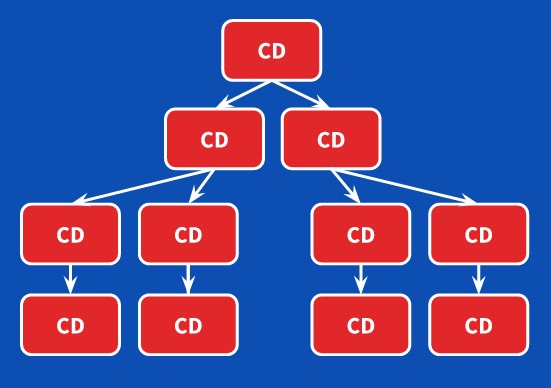
\includegraphics[width=0.7\linewidth]{kapitel3/cd-tree.jpg}
 \caption{Change Detection Flow}\cite{changedetection-explained}
\end{figure}


\section{Ionic}
\subsection{Allgemein}
\subsection{Komponenten verwenden}
\subsection{Deployment}

\section{Electron}
\subsection{Allgemein}
